\documentclass{beamer}
\usepackage[style=numeric]{biblatex}
\usepackage{listings}
\usepackage{inter}
% \usepackage{minted}
% set up coloring
\usepackage{xcolor}
\definecolor{kosovoorange}{RGB}{237, 93, 93}
\definecolor{kosovoblue}{RGB}{0, 73, 255}

% beamer setup
% Choose your desired theme
\usetheme{Hannover}
% use color defined above
\usecolortheme[named=kosovoorange]{structure}

\addbibresource{./cabi.bib}
\title{Pedaling Towards Progress}
\subtitle{Analyzing Washington, DC's Bikesharing system using Open-source tools}
\author{Maxwell Lindsay}
\institute{Van Oord}
\date{\today}
\titlegraphic{
\includegraphics[height=.3\textheight]{./FOSS4G 2023 - Logo Main.png}}
\begin{document}

\begin{frame}
    % 
\includegraphics{./FOSS4G 2023 - Logo Main.png}
    \titlepage
\end{frame}
\section{Introduction}
% \subsection{Who am I?}
\begin{frame}
    \frametitle{About me}
    \begin{itemize}
        \item Originally from Washington, DC area
              % hence my obcession with DC bike infrastructure
        \item Background in Coastal Engineering
        \item Currently work as a Geospatial Developer at Van Oord, In Rotterdam, The Netherlands
    \end{itemize}
    \begin{center}
        
\includegraphics[width=0.4\textwidth]{VO_logo.png}
    \end{center}
\end{frame}

% \subsection{What is Capital Bikeshare?}
\begin{frame}
    % consider splitting into a few slides with more pictures
    \frametitle{Capital Bikeshare basics}
    \begin{columns}
        \column{0.5\textwidth}
        \begin{figure}
            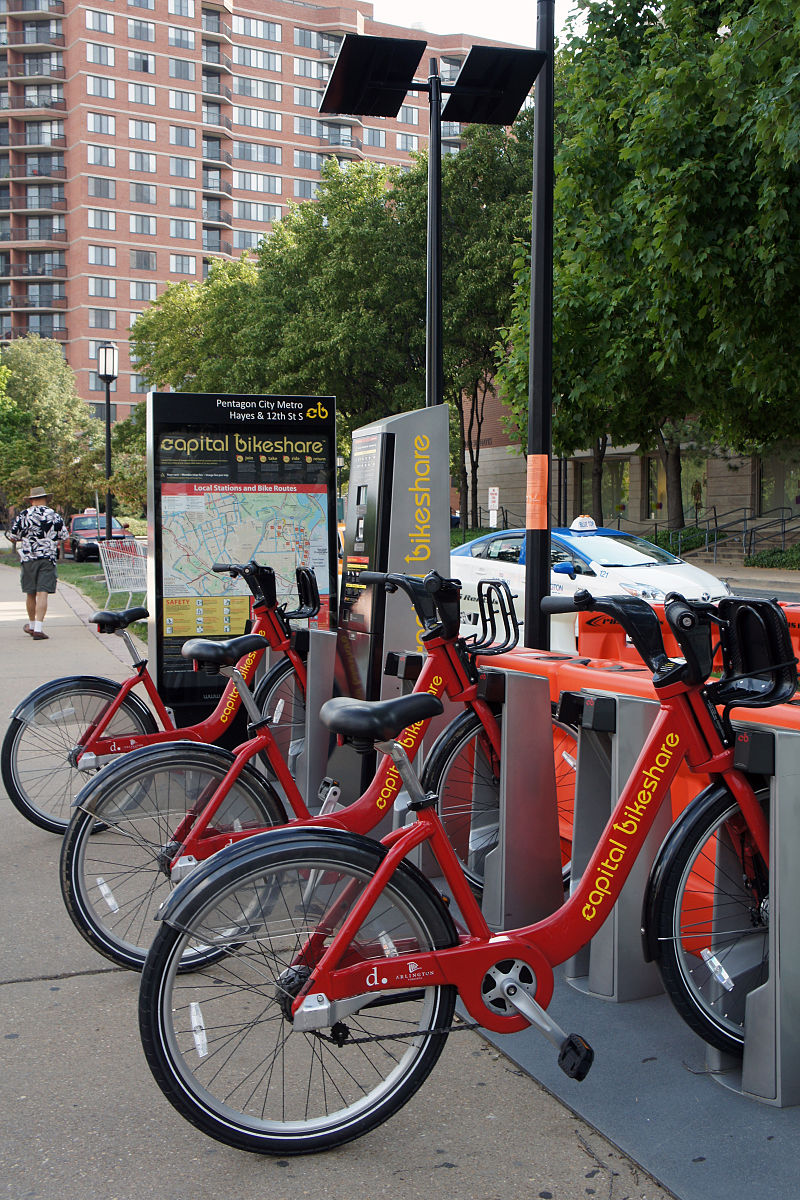
\includegraphics[]{800px-VA_07_2012_Capital_Bikeshare_4152.JPG}
            % \caption{By Mariordo (Mario Roberto Durán Ortiz) - Own work, CC BY-SA 3.0, https://commons.wikimedia.org/w/index.php?curid=20462784}
        \end{figure}
        \column{0.5\textwidth}
        \begin{itemize}
            \item Docked bikeshare
                  % \item Memberships are available for \$95 a year for unlimited trips under 45 minutes \cite{cabisite}. Casual users can pay \$1 to unlock the bike, then \$0.05 per minute.
            \item Primarily intended for short trips
            \item 700+ docking stations
            \item $\approx$ 35 million trips (so far)
        \end{itemize}

    \end{columns}
    % \small{* recently, non-docked E-bikes that have been introduced}
\end{frame}

\begin{frame}
    \frametitle{The current station map}
    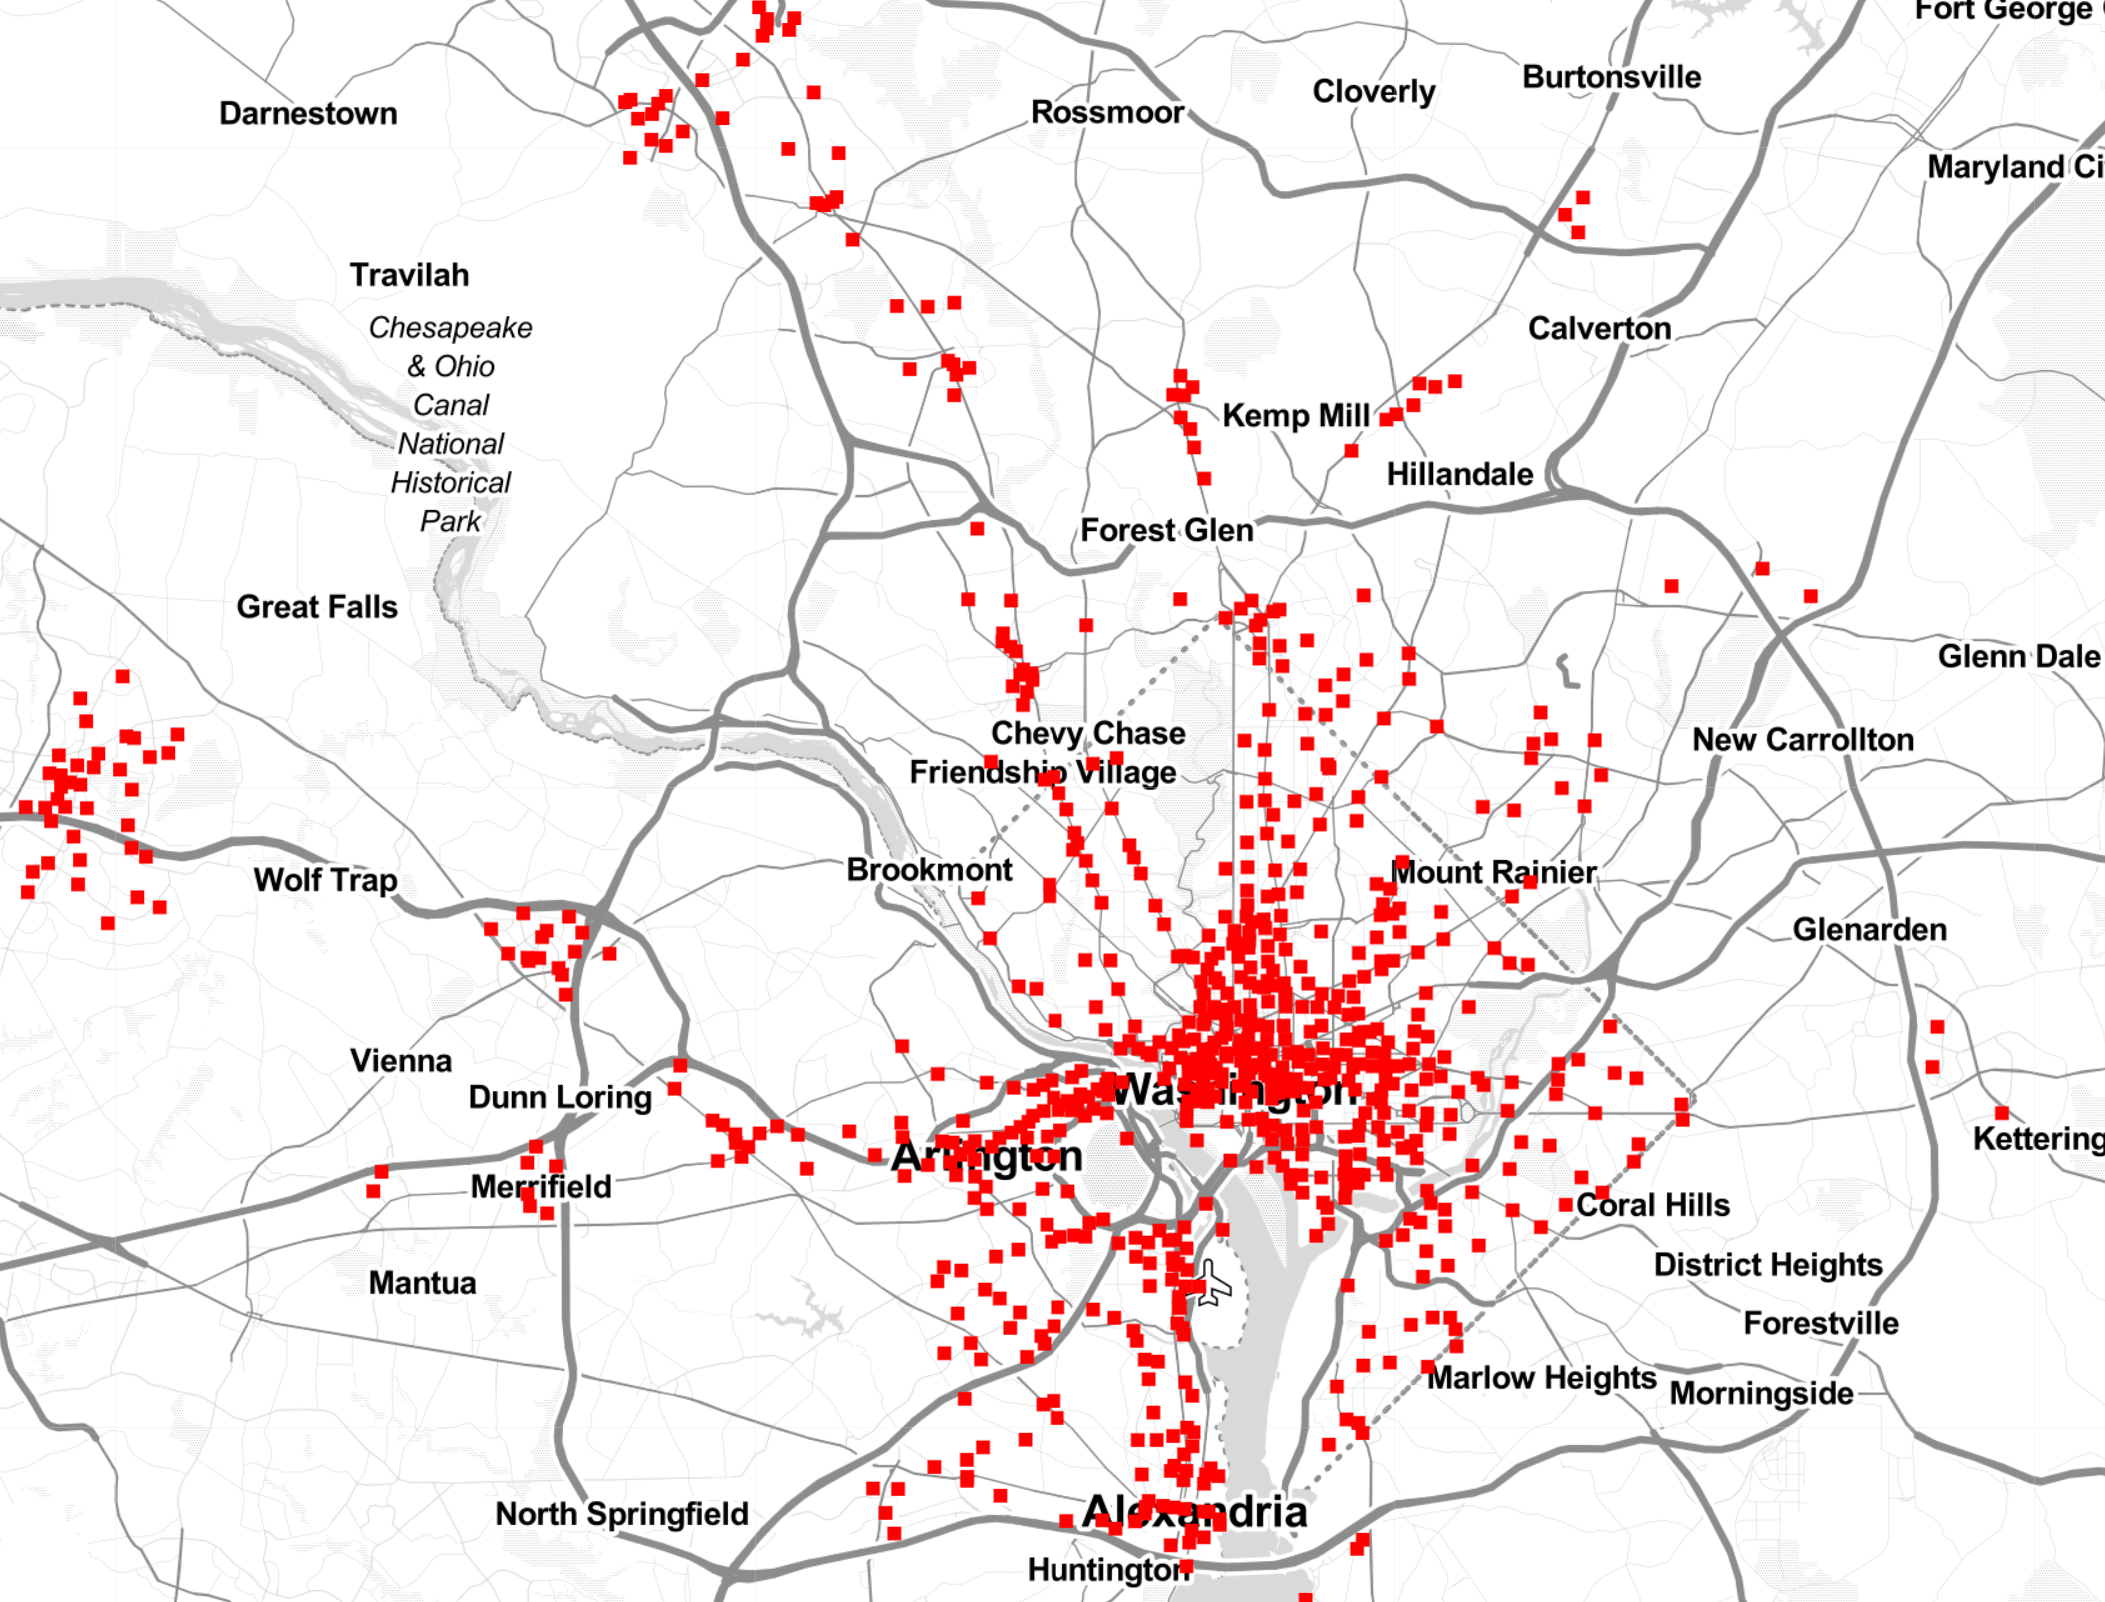
\includegraphics[width=\textwidth]{./cabi_stations.png}
\end{frame}
\begin{frame}
    \frametitle{The data}

    Capital Bikeshare publishes the following data about each trip on a monthly basis:

    \begin{itemize}
        \item start time
        \item end time
        \item start station index
        \item end station index
        \item Membership status of the rider (Member or Non-member?)
    \end{itemize}

    These data are available as csv files per month or year from Capital Bikeshare at https://ride.capitalbikeshare.com/system-data
\end{frame}

\begin{frame}
    \frametitle{Example data}
    % TODO fix this mess
    The raw CSV files are available from the Capital Bikeshare Data portal. This is a small example what the data looks like
    \begin{table}[]
        \begin{tabular}{lllllllllllll}
            \hline
            \multicolumn{1}{|l|}{ride\_id} & \multicolumn{1}{l|}{rideable\_type} & \multicolumn{1}{l|}{started\_at} & \multicolumn{1}{l|}{ended\_at} & \multicolumn{1}{l|}{start\_station\_name} & \multicolumn{1}{l|}{start\_station\_id} & \multicolumn{1}{l|}{end\_station\_name} & \multicolumn{1}{l|}{end\_station\_id} & \multicolumn{1}{l|}{start\_lat} & \multicolumn{1}{l|}{start\_lng} & \multicolumn{1}{l|}{end\_lat} & \multicolumn{1}{l|}{end\_lng} & \multicolumn{1}{l|}{member\_casual} \\ \hline
            5F3D280238A782FE               & docked\_bike                        & 2023-05-12 18:57:59              & 2023-05-12 19:17:50            & 3rd \& Tingey St SE                       & 31634                                   & 8th \& F St NE                          & 31631                                 & 38.87501                        & -77.0024                        & 38.897274                     & -76.994749                    & casual                              \\
            97EC218DACB24849               & classic\_bike                       & 2023-05-23 07:55:29              & 2023-05-23 08:11:12            & Clarendon Blvd \& Pierce St               & 31016                                   & 15th \& L St NW                         & 31276                                 & 38.893438                       & -77.076389                      & 38.903649                     & -77.034918                    & member                              \\
            31D19AC7BA317018               & electric\_bike                      & 2023-05-05 17:27:10              & 2023-05-05 17:40:17            & South Capitol St and Southern Ave SE      & 31830                                   & Tanger Outlets                          & 32415                                 & 38.821667433                    & -77.001627445                   & 38.7968                       & -77.0026                      & member
        \end{tabular}
    \end{table}
\end{frame}

\section{My Goals}
\begin{frame}
    \frametitle{Goal 1}

    Count how many trips ocurred on every unique combination of stations

\end{frame}

\begin{frame}
    \frametitle{Goal 2}

    Find the route of this each of these trips

\end{frame}
\begin{frame}
    \frametitle{Goal 3}
    Combine these two items to get a map of the estimated number of bikeshare trips on every street/road/path in the city
\end{frame}


\begin{frame}
    \frametitle{The Challenges}
    \begin{itemize}
        \item Efficiently putting hundreds of thousands of trips through a routing engine
        \item How to combine these hundreds any thousands of complex multiline geometries to sum the trips on each part (without melting my laptop)
    \end{itemize}
\end{frame}

\section{My Approach}

\begin{frame}
    \frametitle{Overview of my approach}
    \begin{enumerate}
        \item Download all CSV files for all trips
        \item Parse and normalize the CSVs using Pandas
        \item Find The number of trips between unique pairs of stations
        \item Build Valhalla routing tiles
        \item Find a route between each station pair using Valhalla
        \item Aggregate the trip statistics across every single route
    \end{enumerate}
\end{frame}

\begin{frame}
    \frametitle{Data cleaning and validation}
    For each trip, the trip time is calculated.
    Trips are considered invalid based on the following criteria:
    \begin{itemize}
        \item Longer than a 4 hours

              % This is an arbitrary threshold. However, the CaBi system is primarily intended for short trips, and the pricing reflects this. The bikes can be used for leisure and tourism, but they are priced to encourage users to change bikes regularly. Also, for the purposes of this project, long trips are less likely to have

        \item Starting and ending at the same station

              % For obvious reasons, cannot easily be routed

        \item Stations with an invalid start or end station

              % A number of trips in the dataset are missing a value for the start or ending point
    \end{itemize}
    As of May 2023 there are 35,231,413 trips. 175,603 are longer than 4 hours and are removed.
\end{frame}

%\subsection{Find The number of trips between unique pairs of stations}
\begin{frame}
    \frametitle{Find unique trips between station pairs}
    $$ 35,136,810 \text{ trips} \rightarrow 183,959 \text{ station combinations} $$
    If we drop trips that start and end at the same dock, we are down to 183,214 trips.
    \smallskip
    If we consider only \emph{which two} stations are invovled:
    % ie A->B is combined with B->A
    $$ 183,214 \rightarrow 105,636 $$
    \emph{These trips are the final ones to route}
\end{frame}

\begin{frame}
    \frametitle{Find the number of trips between any 2 stations}

    Implemented by looping over the individual trips in a Pandas DataFrame.
\end{frame}
\begin{frame}
    \frametitle{Results of trips between stations}
    \includegraphics[width=\textwidth]{./cabi_with_number_of_trips.png}
\end{frame}
\begin{frame}
    \frametitle{Building a routing network from OSM data}
    \begin{itemize}
        \item Download the OSM data export from geoFabrik in protobuffer format
        \item Trim and merge the protobuf OSM files
        \item Let Valhalla Docker container build the routing tiles automatically 
              % \item Use Pandas the start and end point of every unique trip
    \end{itemize}
\end{frame}
\begin{frame}
    \frametitle{Routing these trips}
    \framesubtitle{Back to Goal 2}
    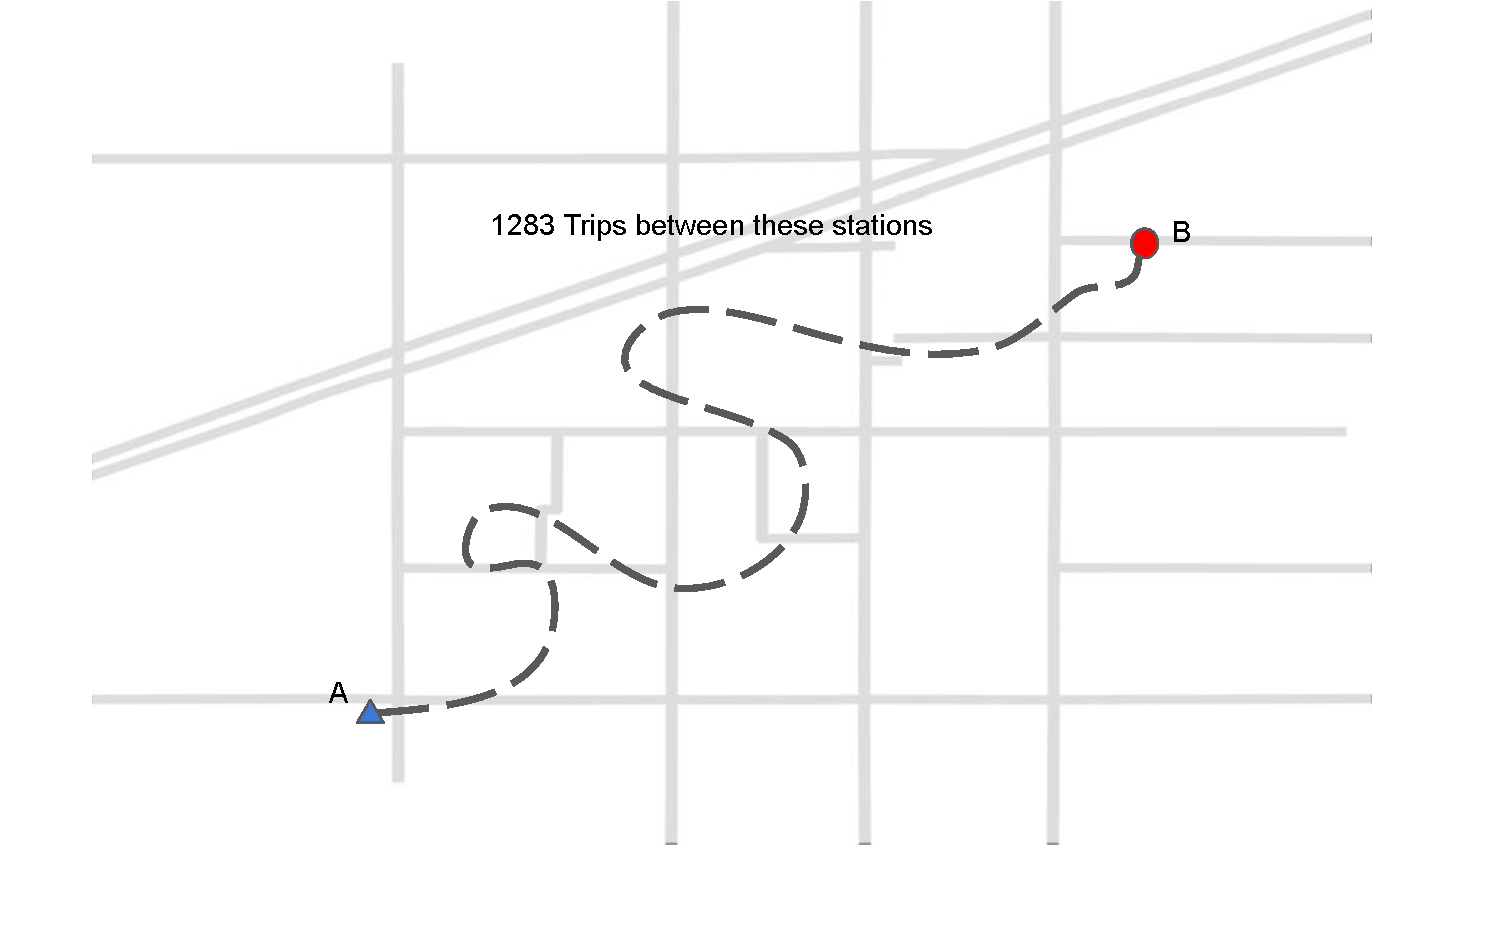
\includegraphics[width=\textwidth,page=1]{graphics_document.pdf}
\end{frame}
\begin{frame}
    \includegraphics[width=\textwidth,page=2]{graphics_document.pdf}
\end{frame}
\begin{frame}
    \includegraphics[width=\textwidth,page=3]{graphics_document.pdf}
\end{frame}
\begin{frame}
    \frametitle{Bike Routing Considerations}
    % \pause
    Vallhalla allows very granular control over bicycle routing, allowing us to set parameters for a cyclist's:
    \begin{itemize}
        \item Bicycle Type\pause
        \item Willingness to share roads with cars\pause
        \item Willingness to bike up hills\pause
        \item Average cycling speed\pause
    \end{itemize} \pause
    How to do this efficiently?\pause 
    \\
    Avoid the Valhalla HTTP API and use \emph{pyvalhalla} 
\end{frame}

\begin{frame}
    \frametitle{Back to Goal 3}
    \framesubtitle{How to combine it all}

    The challenge: \pause
    \\
    How to join over 100k linestrings, summing a certain value \emph{only where they overlap} \pause
    \\
    
    The solution I found: \pause
    \\
    \emph{TopoGeometry}
\end{frame}
\begin{frame}
    \includegraphics[width=\textwidth,page=4]{graphics_document.pdf}
\end{frame}
\begin{frame}
    \includegraphics[width=\textwidth,page=5]{graphics_document.pdf}
\end{frame}
\begin{frame}
    \includegraphics[width=\textwidth,page=6]{graphics_document.pdf}
\end{frame}
\begin{frame}
    \frametitle{PostGIS topology}
    \begin{itemize}
        \item Using PLpgSQL triggers, add a corresponding entry to the topogeometry table for every new entry to the routes tables
    \end{itemize}
\end{frame}

\begin{frame}
    \includegraphics[width=\textwidth,page=7]{graphics_document.pdf}
\end{frame}

\begin{frame}
    \frametitle{Sum up the trips on every topological edge}
    \begin{itemize}
        \item Using an SQL query, we can sum the trips on every unique "section" of road in DC

    \end{itemize}
\end{frame}
\begin{frame}
    \includegraphics[width=\textwidth,page=8]{graphics_document.pdf}
\end{frame}
\begin{frame}
    \includegraphics[width=\textwidth,page=9]{graphics_document.pdf}
\end{frame}
\begin{frame}
    \includegraphics[width=\textwidth,page=10]{graphics_document.pdf}
\end{frame}
\begin{frame}
    \frametitle{The actual implementation}

    \begin{itemize}
        \item<1-> PostGIS hosted inside a Docker container 
        % \item I define a Docker compose file which also includes a Valhalla container. The routing is not hosted in this container (too slow), but every time the app is launched it checks for new OSM data and rebuilds the tiles if needed
        \item<2-> A series of Python scripts load the data, and run the routing software
        \item<3-> Makefile ties everything together
              % reruns just the parts needed, based on what changes have been made Is using Makefiles, in the year of our lord 2023, still good practice? I'm not sure. The syntax is byzantine. I'm absuing it for something it was never intended for. But I still have never found anything that replicates its exact functionality. 
    \end{itemize}

\end{frame}
\section{Results}
\begin{frame}
    \frametitle{Results}
    \includegraphics[width=\textwidth]{./network_stats.jpg}
\end{frame}
\begin{frame}
    \frametitle{Validation}
    \framesubtitle{How accurate is this?}

    Are the sums for any individual routes anywhere near accurate? \pause
    \\
    \emph{Probably not?}
    % Probably not. However, I would speculate that the ratios \emph{between} streets are probably more representative.

    % The only validation data I know of (GPS Tracks collected during a study in 2016) are not public and I'm still working on getting access to them.
\end{frame}
\section{Takeaways}

\begin{frame}
    \frametitle{Which steps made this practical to run on a laptop?}

    \begin{itemize}
        % \item If you don't need a web API, use \emph{pyvalhalla} for much faster interaction with the routing engine
        \item using \emph{pyvalhalla} instead of hosting it in Docker
        \item Using topology to sum trips by street
        % \item Using SQL triggers allows the topogeometry to be built as you add geometry to the database
        \item Using SQL triggers for creating the topogeometry 
    \end{itemize}
\end{frame}
\begin{frame}
    \frametitle{What would I have done differently?}

    \begin{itemize}
        \item More in SQL, less in Python
        \item Python is perfect for being the "Glue" and interacting with the various parts
              % If I was starting from scratch, I would probably move a lot of the other logic to PostGIS, and use SQL queries and functions to do more of the data crunching

    \end{itemize}
\end{frame}

\section{Thanks}

\begin{frame}
    \frametitle{Shoutouts}

\includegraphics[width=\textwidth]{logos_thanks.png}
\end{frame}
\begin{frame}
    Thanks for your interest
\end{frame}
\end{document}
